\documentclass[11pt,a4paper]{article}

% --- Packages ---
\usepackage[margin=1in]{geometry}
\usepackage{amsmath,amssymb,amsfonts}
\usepackage{graphicx}
\usepackage[american]{circuitikz}
\usepackage{booktabs}
\usepackage{subcaption}
\usepackage{float}
\usepackage{parskip}
\usepackage{microtype}
\usepackage[colorlinks=true,linkcolor=blue,citecolor=blue,urlcolor=blue]{hyperref}
\usepackage{titlesec}

% --- Section Styling ---
\titleformat{\section}{\large\bfseries}{\thesection}{1em}{}
\titleformat{\subsection}{\normalsize\bfseries}{\thesubsection}{1em}{}

% --- Title block ---
\title{
    \vspace{-1.5cm}
    \textbf{\Large 6. Op-Amp: Square, Triangular \& Sawtooth wave generators:} \\
    \vspace{0.3cm}
    \large Advanced Physics Laboratory II (PHY325)
}
\author{}
\date{}

\begin{document}

\maketitle
\vspace{-1.5cm}
\begin{center}
    \renewcommand{\arraystretch}{1.2}
    \begin{tabular}{ll@{\hspace{1cm}}ll}
        \textbf{Name:} & Yamulapalli Nandu Navadeep & \textbf{Date of Experiment:} & 27/07/2026 \\
        \textbf{Roll No:} & IMS24267 & \textbf{Date of Submission:} & 03/08/2026 \\
        \textbf{Group No:} & 6 & & \\
    \end{tabular}
\end{center}
\vspace{0.3cm}
\hrule
\vspace{0.3cm}

% ==========================================
% 1. AIM
% ==========================================
\section{Aim}
To set up and study the square, triangular and saw-tooth waveform generators using IC 741.
% ==========================================
% 2. COMPONENTS REQUIRED
% ==========================================
\section{Components Required}
The components and equipment required for this experiment are listed in Table~\ref{tab:components}.

\begin{table}[H]
\centering
\caption{List of Required Components and Instrumentation}
\label{tab:components}
\begin{tabular}{llc}
\toprule
\textbf{Component / Instrument} & \textbf{Specification / Value} & \textbf{Quantity} \\
\midrule
Operational Amplifier & IC 741 & 2 \\
Resistors & $4.7\text{ k}\Omega$ & 4 \\
 & $33\text{ k}\Omega$ & 1 \\
 & $220\text{ k}\Omega$ (Bleeding Resistor) & 1 \\
Capacitors & $0.47\ \mu\text{F}$ & 2 \\
Variable Resistor & Potentiometer ($10\text{ k}\Omega$) & 1 \\
Power Supply & Dual Tracking DC Power Supply ($\pm 15\text{V}$) & 1 \\
Measuring Instruments & Digital Storage Oscilloscope (DSO) with Probes & 1 \\
Prototyping & Solderless Breadboard and Connecting Wires & 1 \\
\bottomrule
\end{tabular}
\end{table}

% ==========================================
% 3. THEORY & CIRCUIT DIAGRAMS
% ==========================================
\section{Theory and Circuit Design}

\subsection{Square Wave Generator}
An op-amp can be configured as a square wave generator (astable multivibrator) using simultaneous positive and negative feedback loops, as shown in Figure~\ref{fig:square_circ}. A voltage divider made of two equal $4.7\text{ k}\Omega$ resistors ($R_1$ and $R_2$) at the non-inverting terminal (+) sets the reference trigger voltages ($\pm V_{\text{threshold}}$). An $RC$ timing network at the inverting terminal (-) determines the oscillation time period.

The capacitor $C$ repeatedly charges and discharges toward the op-amp output saturation voltages ($\pm V_{\text{sat}}$). When the voltage across the capacitor crosses the threshold voltage at the non-inverting terminal, the op-amp comparator action forces the output to rapidly switch to the opposite saturation state. This continuous switching produces a steady square wave at the output terminal (Pin 6).

\begin{figure}[H]
\centering
\begin{circuitikz}[scale=0.95, transform shape]
    % Main op-amp
    \draw (0,0) node[op amp] (op) {};
    
    % Pin labels near terminal
    \node[right, font=\scriptsize] at (op.-) {2};
    \node[right, font=\scriptsize] at (op.+) {3};
    \node[above left, font=\scriptsize] at (op.out) {6};
    \node[below, font=\scriptsize] at (op.up) {7};
    \node[above, font=\scriptsize] at (op.down) {4};
    
    % Power supply connections
    \draw (op.up) -- ++(0,0.5) node[vcc]{$+15\text{V}$};
    \draw (op.down) -- ++(0,-0.5) node[vee]{$-15\text{V}$};
    
    % Output node and wire
    \draw (op.out) -- ++(1,0) coordinate (out_junct) to[short, -o] ++(1.5,0) node[right, font=\bfseries]{Square Wave Output};
    
    % Negative feedback loop (Timing Network: upper loop)
    \draw (out_junct) -- ++(0, 2.2) coordinate (top_f) 
          to[R, l_=$4.7\text{ k}\Omega$ ($R$)] ++(-5.0, 0) coordinate (top_in)
          -- (top_in |- op.-) -- (op.-);
    % Capacitor from Pin 2 to Ground (horizontal)
    \draw (top_in |- op.-) to[C, l=$0.47\ \mu\text{F}$ ($C$), *-] ++(-3.2,0) -- ++(0,-0.6) node[ground]{};
          
    % Positive feedback loop (Voltage Divider: lower loop)
    \draw (out_junct) -- ++(0, -2.2) coordinate (bot_f)
          to[R, l=$4.7\text{ k}\Omega$ ($R_1$)] ++(-5.0, 0) coordinate (bot_in)
          -- (bot_in |- op.+) -- (op.+);
          
    % Resistor R2 from Pin 3 to Ground
    \draw (bot_in |- op.+) -- ++(-1.5,0) coordinate (r2_node)
          to[R, l=$4.7\text{ k}\Omega$ ($R_2$)] (r2_node |- 0,-2.6) node[ground]{};
\end{circuitikz}
\caption{Circuit Diagram 1: Square Wave Generator using an IC 741 op-amp.}
\label{fig:square_circ}
\end{figure}

For a symmetrical voltage divider where $R_1 = R_2$, the switching thresholds are at $\pm \frac{1}{2} V_{\text{sat}}$, and the theoretical oscillation frequency $f$ is given by:
\begin{equation}
    f \approx \frac{1}{2.2 \, R \, C}
    \label{eq:freq}
\end{equation}
Substituting the experimental component values ($R = 4.7\text{ k}\Omega$ and $C = 0.47\ \mu\text{F}$), the theoretical time period $T_{\text{theo}}$ and fundamental oscillation frequency $f_{\text{theo}}$ are calculated as:
\begin{align}
    T_{\text{theo}} &\approx 2.2 \, R \, C \approx 2.2 \times (4.7 \times 10^3\ \Omega) \times (0.47 \times 10^{-6}\ \text{F}) \approx 4.86\text{ ms} \label{eq:theo_period} \\
    f_{\text{theo}} &= \frac{1}{T_{\text{theo}}} \approx \frac{1}{4.86 \times 10^{-3}\ \text{s}} \approx 205.7\text{ Hz} \label{eq:theo_freq}
\end{align}

---

\subsection{Triangle Wave Generator (Integrator)}
Integrating a constant voltage over time results in a steadily rising or falling linear ramp. When the square wave produced by Circuit 1 is fed into an op-amp configured as an integrator (Figure~\ref{fig:triangle_circ}), the feedback capacitor ($C_f$) charges and discharges at a constant rate ($\pm I_{in} = \pm V_{\text{in}} / R_{in}$). This converts the input square wave into a symmetrical triangular waveform at the output.

\begin{figure}[H]
\centering
\begin{circuitikz}[scale=0.95, transform shape]
    % Main op-amp
    \draw (0,0) node[op amp] (op) {};
    
    % Pin labels
    \node[right, font=\scriptsize] at (op.-) {2};
    \node[right, font=\scriptsize] at (op.+) {3};
    \node[above left, font=\scriptsize] at (op.out) {6};
    \node[below, font=\scriptsize] at (op.up) {7};
    \node[above, font=\scriptsize] at (op.down) {4};
    
    % Power supply
    \draw (op.up) -- ++(0,0.5) node[vcc]{$+15\text{V}$};
    \draw (op.down) -- ++(0,-0.5) node[vee]{$-15\text{V}$};
    
    % Input network to Pin 2 (-)
    \draw (-4.5, 0.5) node[anchor=east, font=\bfseries]{Square Wave In} to[short, o-] (-4.0, 0.5)
          to[R, l=$4.7\text{ k}\Omega$ ($R_{in}$)] (-1.8, 0.5)
          -- (op.-);
          
    % Non-inverting Pin 3 (+) directly to Ground
    \draw (op.+) -- ++(0, -1.0) node[ground]{};
    
    % Output network
    \draw (op.out) -- ++(1.5,0) coordinate (out_junct) to[short, -o] ++(1.5,0) node[right, font=\bfseries]{Triangle Wave Output};
    
    % Feedback junction on input side
    \coordinate (in_junct) at (-1.8, 0.5);
    
    % Parallel feedback: Capacitor Cf branch (lower loop)
    \draw (out_junct) -- ++(0, 1.8) coordinate (f_cap_right)
          to[C, l_=$0.47\ \mu\text{F}$ ($C_f$)] (in_junct |- f_cap_right)
          -- (in_junct);
          
    % Parallel feedback: Resistor Rf branch (upper loop)
    \draw (f_cap_right) -- ++(0, 1.3) coordinate (f_res_right)
          to[R, l_=$220\text{ k}\Omega$ ($R_f$)] (in_junct |- f_res_right)
          -- (in_junct |- f_cap_right);
\end{circuitikz}
\caption{Circuit Diagram 2: Triangle Wave Generator (Integrator with resistor $R_f$).}
\label{fig:triangle_circ}
\end{figure}

In a simple integrator circuit, even a tiny input offset voltage can accumulate across the feedback capacitor over time, eventually driving the op-amp output into saturation (clipping against the power supply rails). To prevent this drift, a large resistor ($R_f = 220\text{ k}\Omega$) is connected in parallel with the feedback capacitor ($C_f = 0.47\ \mu\text{F}$). This resistor limits the low-frequency gain and discharges unwanted DC offsets. The output voltage of the integrator is given by:
\begin{equation}
    V_{\text{out}}(t) = -\frac{1}{R_{in} C_f} \int V_{\text{in}}(t) \, dt
    \label{eq:integ}
\end{equation}
Since the integrator operates directly on the incoming square wave, its theoretical time period is identical to that of the input wave:
\begin{equation}
    T_{\text{theo, triangle}} = T_{\text{theo, square}} \approx 4.86\text{ ms} \quad (f_{\text{theo}} \approx 205.7\text{ Hz})
\end{equation}

---

\subsection{Sawtooth Wave Generator}
A sawtooth waveform requires completely unequal charging and discharging rates—for instance, a slow linear voltage increase followed by a rapid downward drop. As shown in Figure~\ref{fig:sawtooth_circ}, this asymmetry is achieved by applying an external DC bias voltage ($V_{\text{bias}}$) to the non-inverting terminal (Pin 3) using a potentiometer connected across the $\pm 15\text{V}$ power supply rails.

\begin{figure}[H]
\centering
\begin{circuitikz}[scale=0.95, transform shape]
    % Main op-amp
    \draw (0,0) node[op amp] (op) {};
    
    % Pin labels
    \node[right, font=\scriptsize] at (op.-) {2};
    \node[right, font=\scriptsize] at (op.+) {3};
    \node[above left, font=\scriptsize] at (op.out) {6};
    \node[below, font=\scriptsize] at (op.up) {7};
    \node[above, font=\scriptsize] at (op.down) {4};
    
    % Power supply
    \draw (op.up) -- ++(0,0.1) node[vcc]{$+15\text{V}$};
    \draw (op.down) -- ++(0,-0.1) node[vee]{$-15\text{V}$};
    
    % Input network to Pin 2 (-) [Note value change to 33k]
    \draw (-4.5, 0.5) node[anchor=east, font=\bfseries]{Square Wave In} to[short, o-] (-4.0, 0.5)
          to[R, l=$33\text{ k}\Omega$ ($R_{in}$)] (-1.8, 0.5)
          -- (op.-);
          
    % Output network
    \draw (op.out) -- ++(1.5,0) coordinate (out_junct) to[short, -o] ++(1.5,0) node[right, font=\bfseries]{Sawtooth Wave Output};
    
    % Feedback junction on input side
    \coordinate (in_junct) at (-1.8, 0.5);
    
    % Parallel feedback: Capacitor Cf branch
    \draw (out_junct) -- ++(0, 2.2) coordinate (f_cap_right)
          to[C, l_=$0.47\ \mu\text{F}$ ($C_f$)] (in_junct |- f_cap_right)
          -- (in_junct);
          
    % Parallel feedback: Resistor Rf branch
    \draw (f_cap_right) -- ++(0, 1.3) coordinate (f_res_right)
          to[R, l_=$220\text{ k}\Omega$ ($R_f$)] (in_junct |- f_res_right)
          -- (in_junct |- f_cap_right);
          
    % Potentiometer DC Bias network at bottom (positioned to the left)
    \draw (-5.2, -2.6) node[vee]{$-15\text{V}$} 
          -- (-4.5, -2.6) 
          to[R, l_=$10\text{ k}\Omega\text{ Potentiometer}$, name=pot] (-0.9, -2.6)
          -- (-0.2, -2.6) node[vcc]{$+15\text{V}$};
          
    % Wiper connection turning left from Pin 3 (+) to potentiometer center
    \draw (op.+) -- (pot.north |- op.+) coordinate (wiper_turn);
    \draw[-latex, thick] (wiper_turn) -- (pot.north) node[midway, left, font=\footnotesize]{};
\end{circuitikz}
\caption{Circuit Diagram 3: Sawtooth Wave Generator with variable DC biasing at Pin 3 and input resistance $R_{in} = 33\text{ k}\Omega$.}
\label{fig:sawtooth_circ}
\end{figure}

Applying a DC bias voltage ($V_{\text{bias}}$) to Pin 3 sets the virtual ground at Pin 2 to the same potential ($V_{\text{inverting}} \approx V_{\text{bias}}$). Because of this offset, the current flowing into the capacitor through $R_{in}$ is significantly different when the incoming square wave is at its positive high state ($+V_{\text{sq}}$) versus its negative low state ($-V_{\text{sq}}$):
\begin{align*}
    I_{\text{charge}} &= \frac{+V_{\text{sq}} - V_{\text{bias}}}{R_{in}} \\
    I_{\text{discharge}} &= \frac{-V_{\text{sq}} - V_{\text{bias}}}{R_{in}}
\end{align*}
When $V_{\text{bias}}$ is shifted away from zero, one current magnitude becomes much larger than the other. This causes the capacitor to charge slowly (forming a gradual linear ramp) and discharge quickly (forming a sharp drop), producing a sawtooth shape. Additionally, the input resistor $R_{in}$ is increased from $4.7\text{ k}\Omega$ to $33\text{ k}\Omega$ to reduce the integration rate so the output voltage does not hit the power supply limits ($\pm 15\text{V}$) and clip.

Even though the charging and discharging rates are unequal, the total time period of each complete cycle is still determined directly by the input square wave:
\begin{equation}
    T_{\text{theo, sawtooth}} = T_{\text{theo, square}} \approx 4.86\text{ ms} \quad (f_{\text{theo}} \approx 205.7\text{ Hz})
\end{equation}

% ==========================================
% 4. PROCEDURE
% ==========================================
\section{Procedure}
\begin{enumerate}
    \item \textbf{Power Supply Setup:} Connect the dual DC power supply to provide $+15\text{V}$, $-15\text{V}$, and Ground to the power rails of the breadboard.
    \item \textbf{Square Wave Generator:} Build the circuit around the first IC 741 op-amp as shown in Circuit Diagram 1 (Figure~\ref{fig:square_circ}). Connect an oscilloscope probe (set to DC coupling) to Pin 6 to observe and verify the generated square wave.
    \item \textbf{Triangle Wave Generator:} Build the integrator circuit on the second IC 741 op-amp (Circuit Diagram 2, Figure~\ref{fig:triangle_circ}). Connect the square wave output from the first circuit to the input of this integrator through a $4.7\text{ k}\Omega$ resistor ($R_{in}$). Include the $220\text{ k}\Omega$ resistor in parallel with the capacitor ($C_f = 0.47\ \mu\text{F}$) to prevent DC drift. Observe and record the triangular waveform at Pin 6.
    \item \textbf{Sawtooth Wave Generator:} Modify the integrator circuit by disconnecting Pin 3 from ground and connecting it to the wiper of a $10\text{ k}\Omega$ potentiometer placed across the $\pm 15\text{V}$ power rails (Circuit Diagram 3, Figure~\ref{fig:sawtooth_circ}). Increase the input resistor ($R_{in}$) from $4.7\text{ k}\Omega$ to $33\text{ k}\Omega$.
    \item \textbf{Adjusting the Waveform:} Slowly rotate the potentiometer wiper to change the DC bias at Pin 3. Observe on the oscilloscope how the output waveform shifts from a symmetrical triangle wave into an asymmetric sawtooth wave.
\end{enumerate}

% ==========================================
% 5. EXPERIMENTAL WAVEFORMS & FIGURES
% ==========================================
\section{Experimental Waveforms}
The circuits were built on a breadboard and tested using a Digital Storage Oscilloscope (DSO). For each circuit, photographs of the hardware setup and the output waveform displayed on the oscilloscope were recorded.


\subsection{Square Wave Circuit}
The first op-amp circuit generated a steady square wave. Figure~\ref{fig:exp_square} shows the physical breadboard setup alongside the waveform displayed on the oscilloscope. The output cleanly alternates between positive and negative voltage levels at a frequency close to the theoretical calculation ($\approx 205\text{ Hz}$).

\begin{figure}[H]
\centering
\begin{subfigure}{0.48\textwidth}
    \centering
    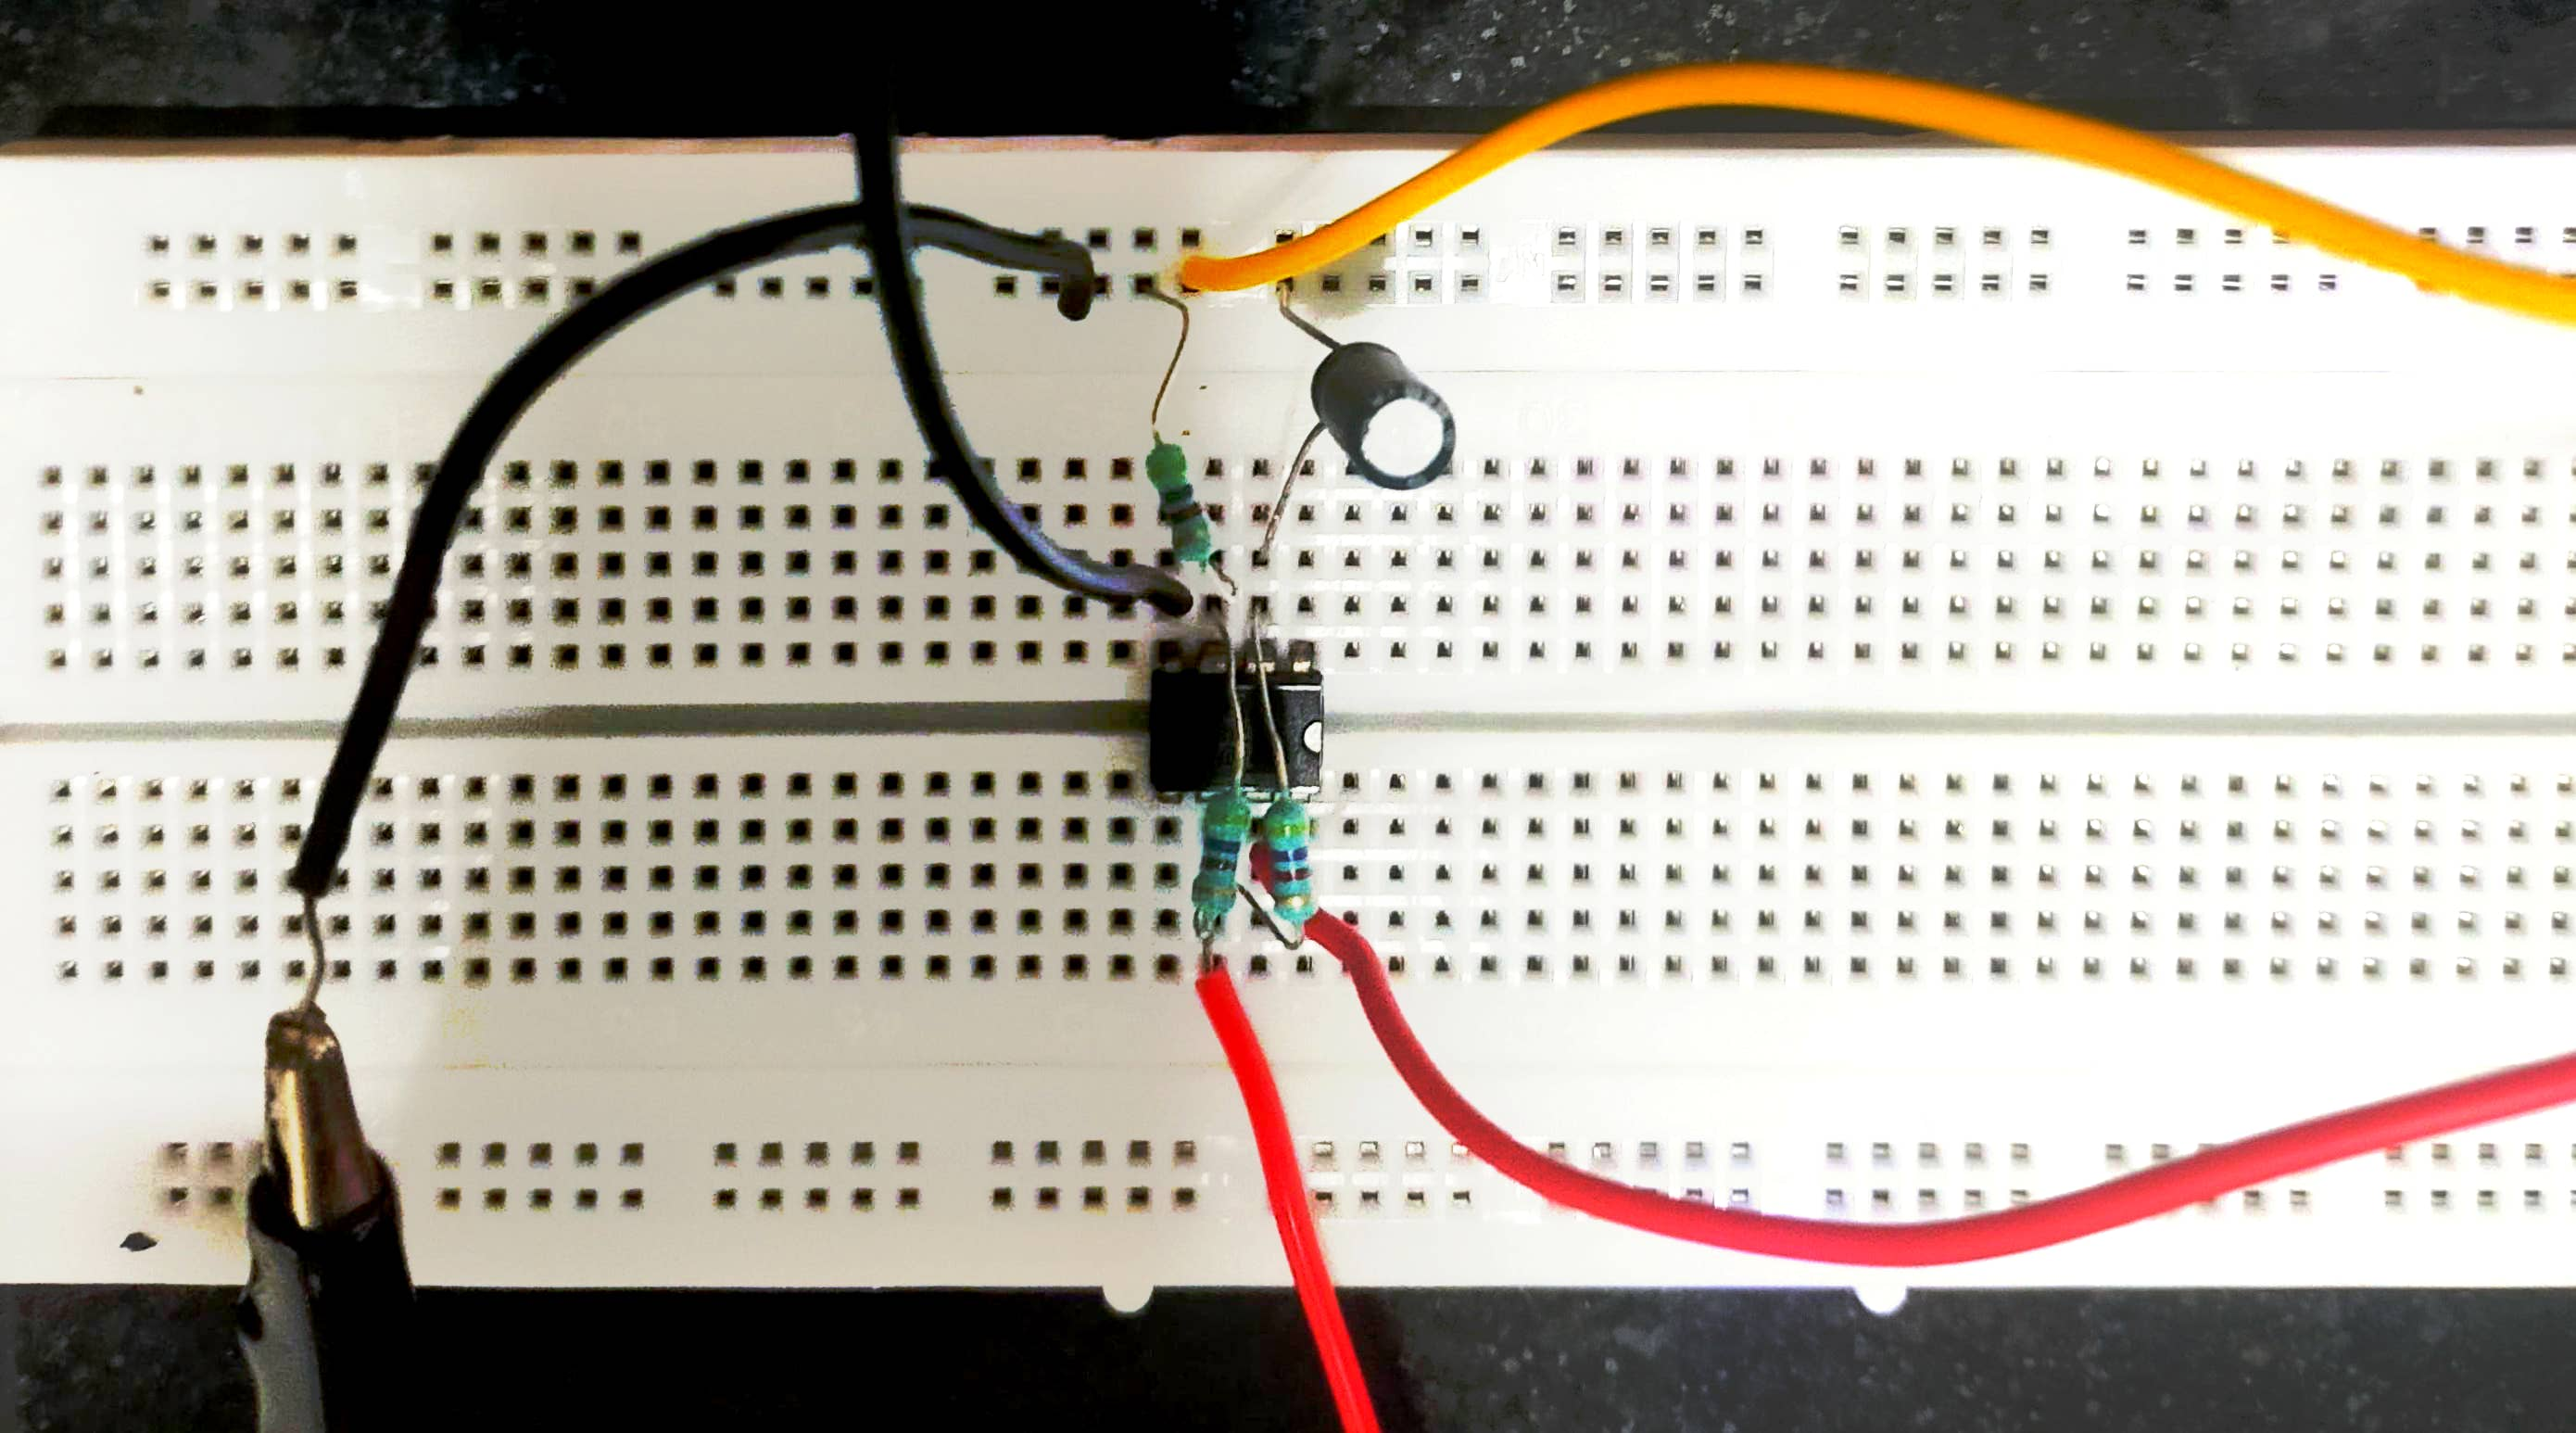
\includegraphics[width=\linewidth]{Images/Square.jpg}
    \caption{Breadboard Circuit Implementation}
    \label{fig:sq_photo}
\end{subfigure}
\hfill
\begin{subfigure}{0.48\textwidth}
    \centering
    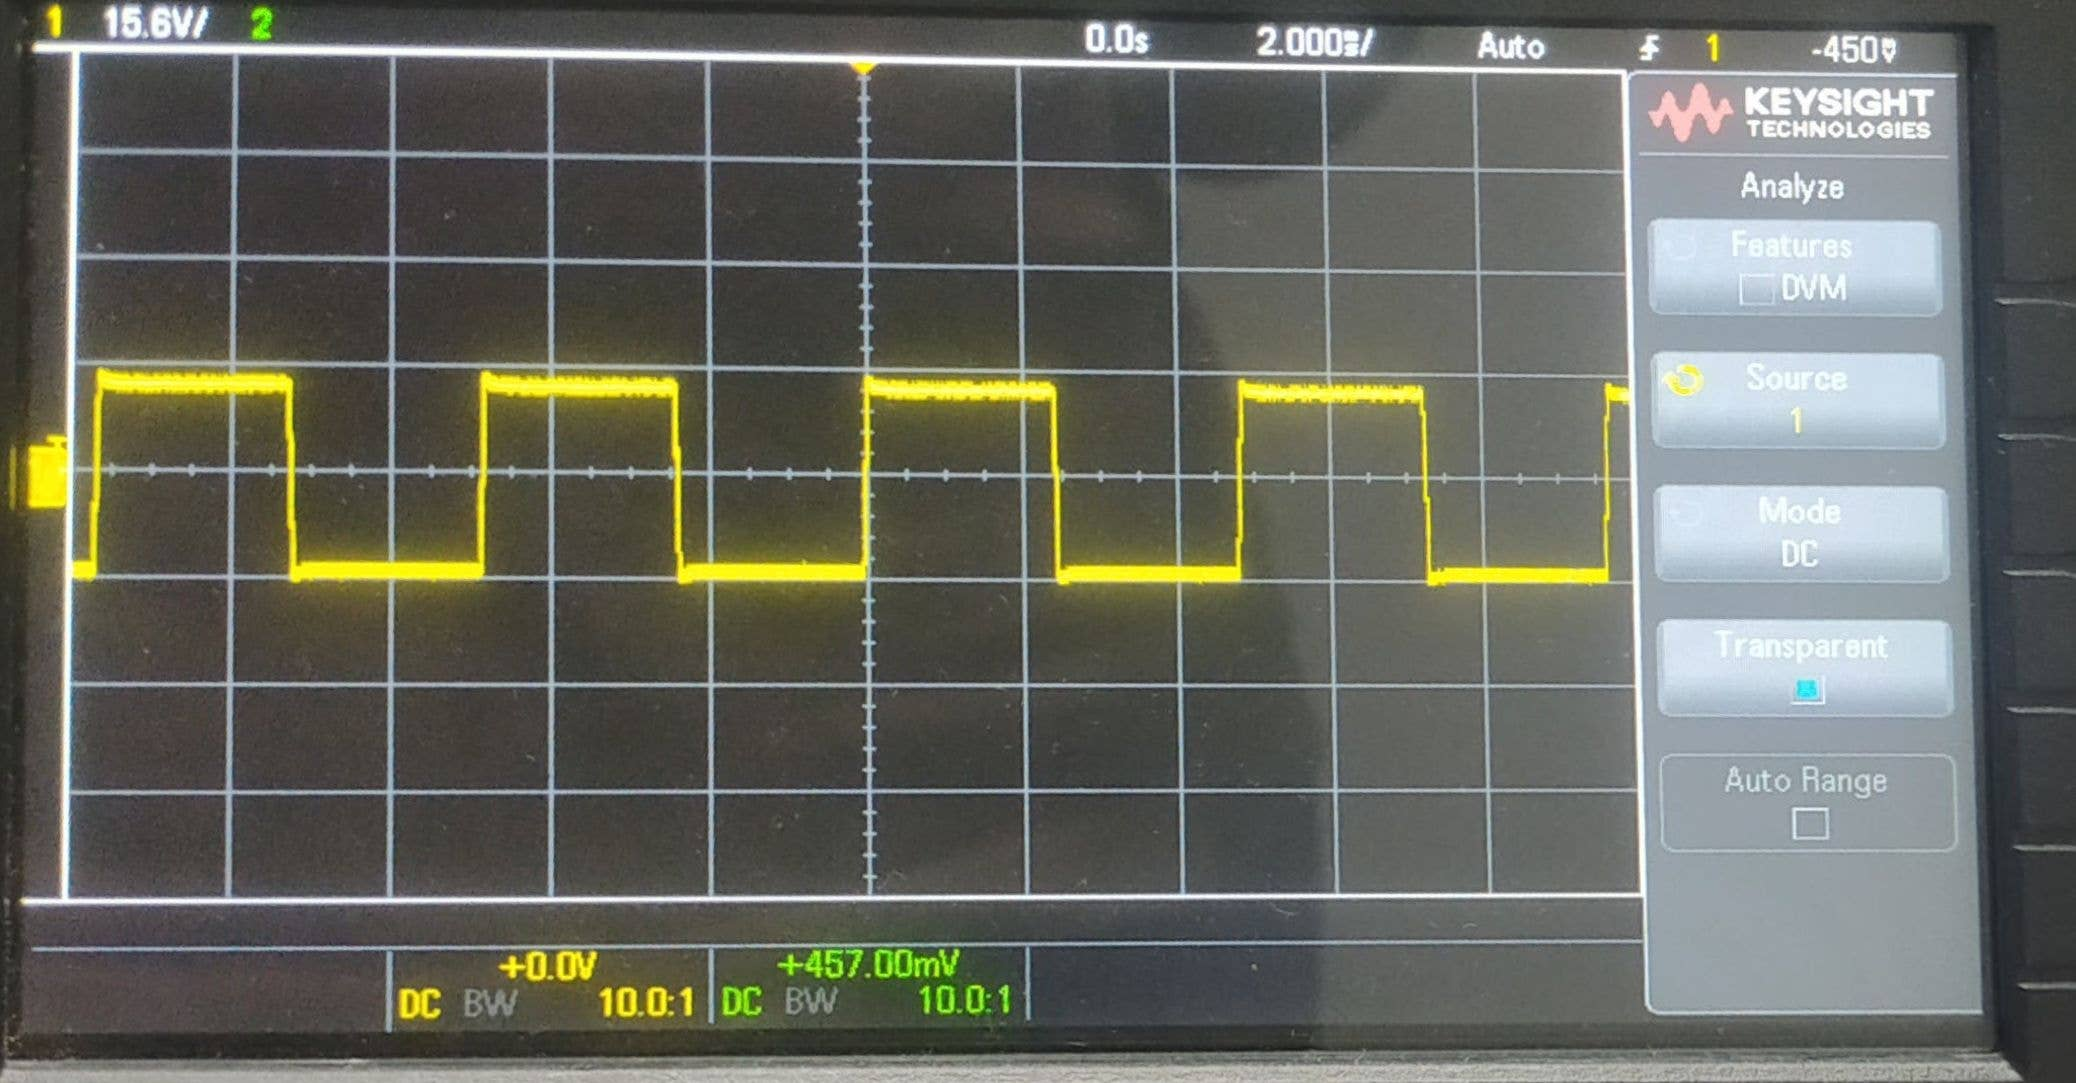
\includegraphics[width=\linewidth]{Images/Graph_Square.jpg}
    \caption{Oscilloscope Signal Capture}
    \label{fig:sq_graph}
\end{subfigure}
\caption{Experimental setup and oscilloscope capture of the square wave generator output at Pin 6.}
\label{fig:exp_square}
\end{figure}

\subsection{Triangular Wave Circuit}
Feeding the square wave into the second op-amp integrator produced a clean triangle wave (Figure~\ref{fig:exp_triangle}). Since the charging current remains constant during each half of the square wave cycle, the output voltage rises and falls in straight linear slopes. The $220\text{ k}\Omega$ feedback resistor prevented offset voltage drift and kept the signal centered around zero volts without clipping.

\begin{figure}[H]
\centering
\begin{subfigure}{0.48\textwidth}
    \centering
    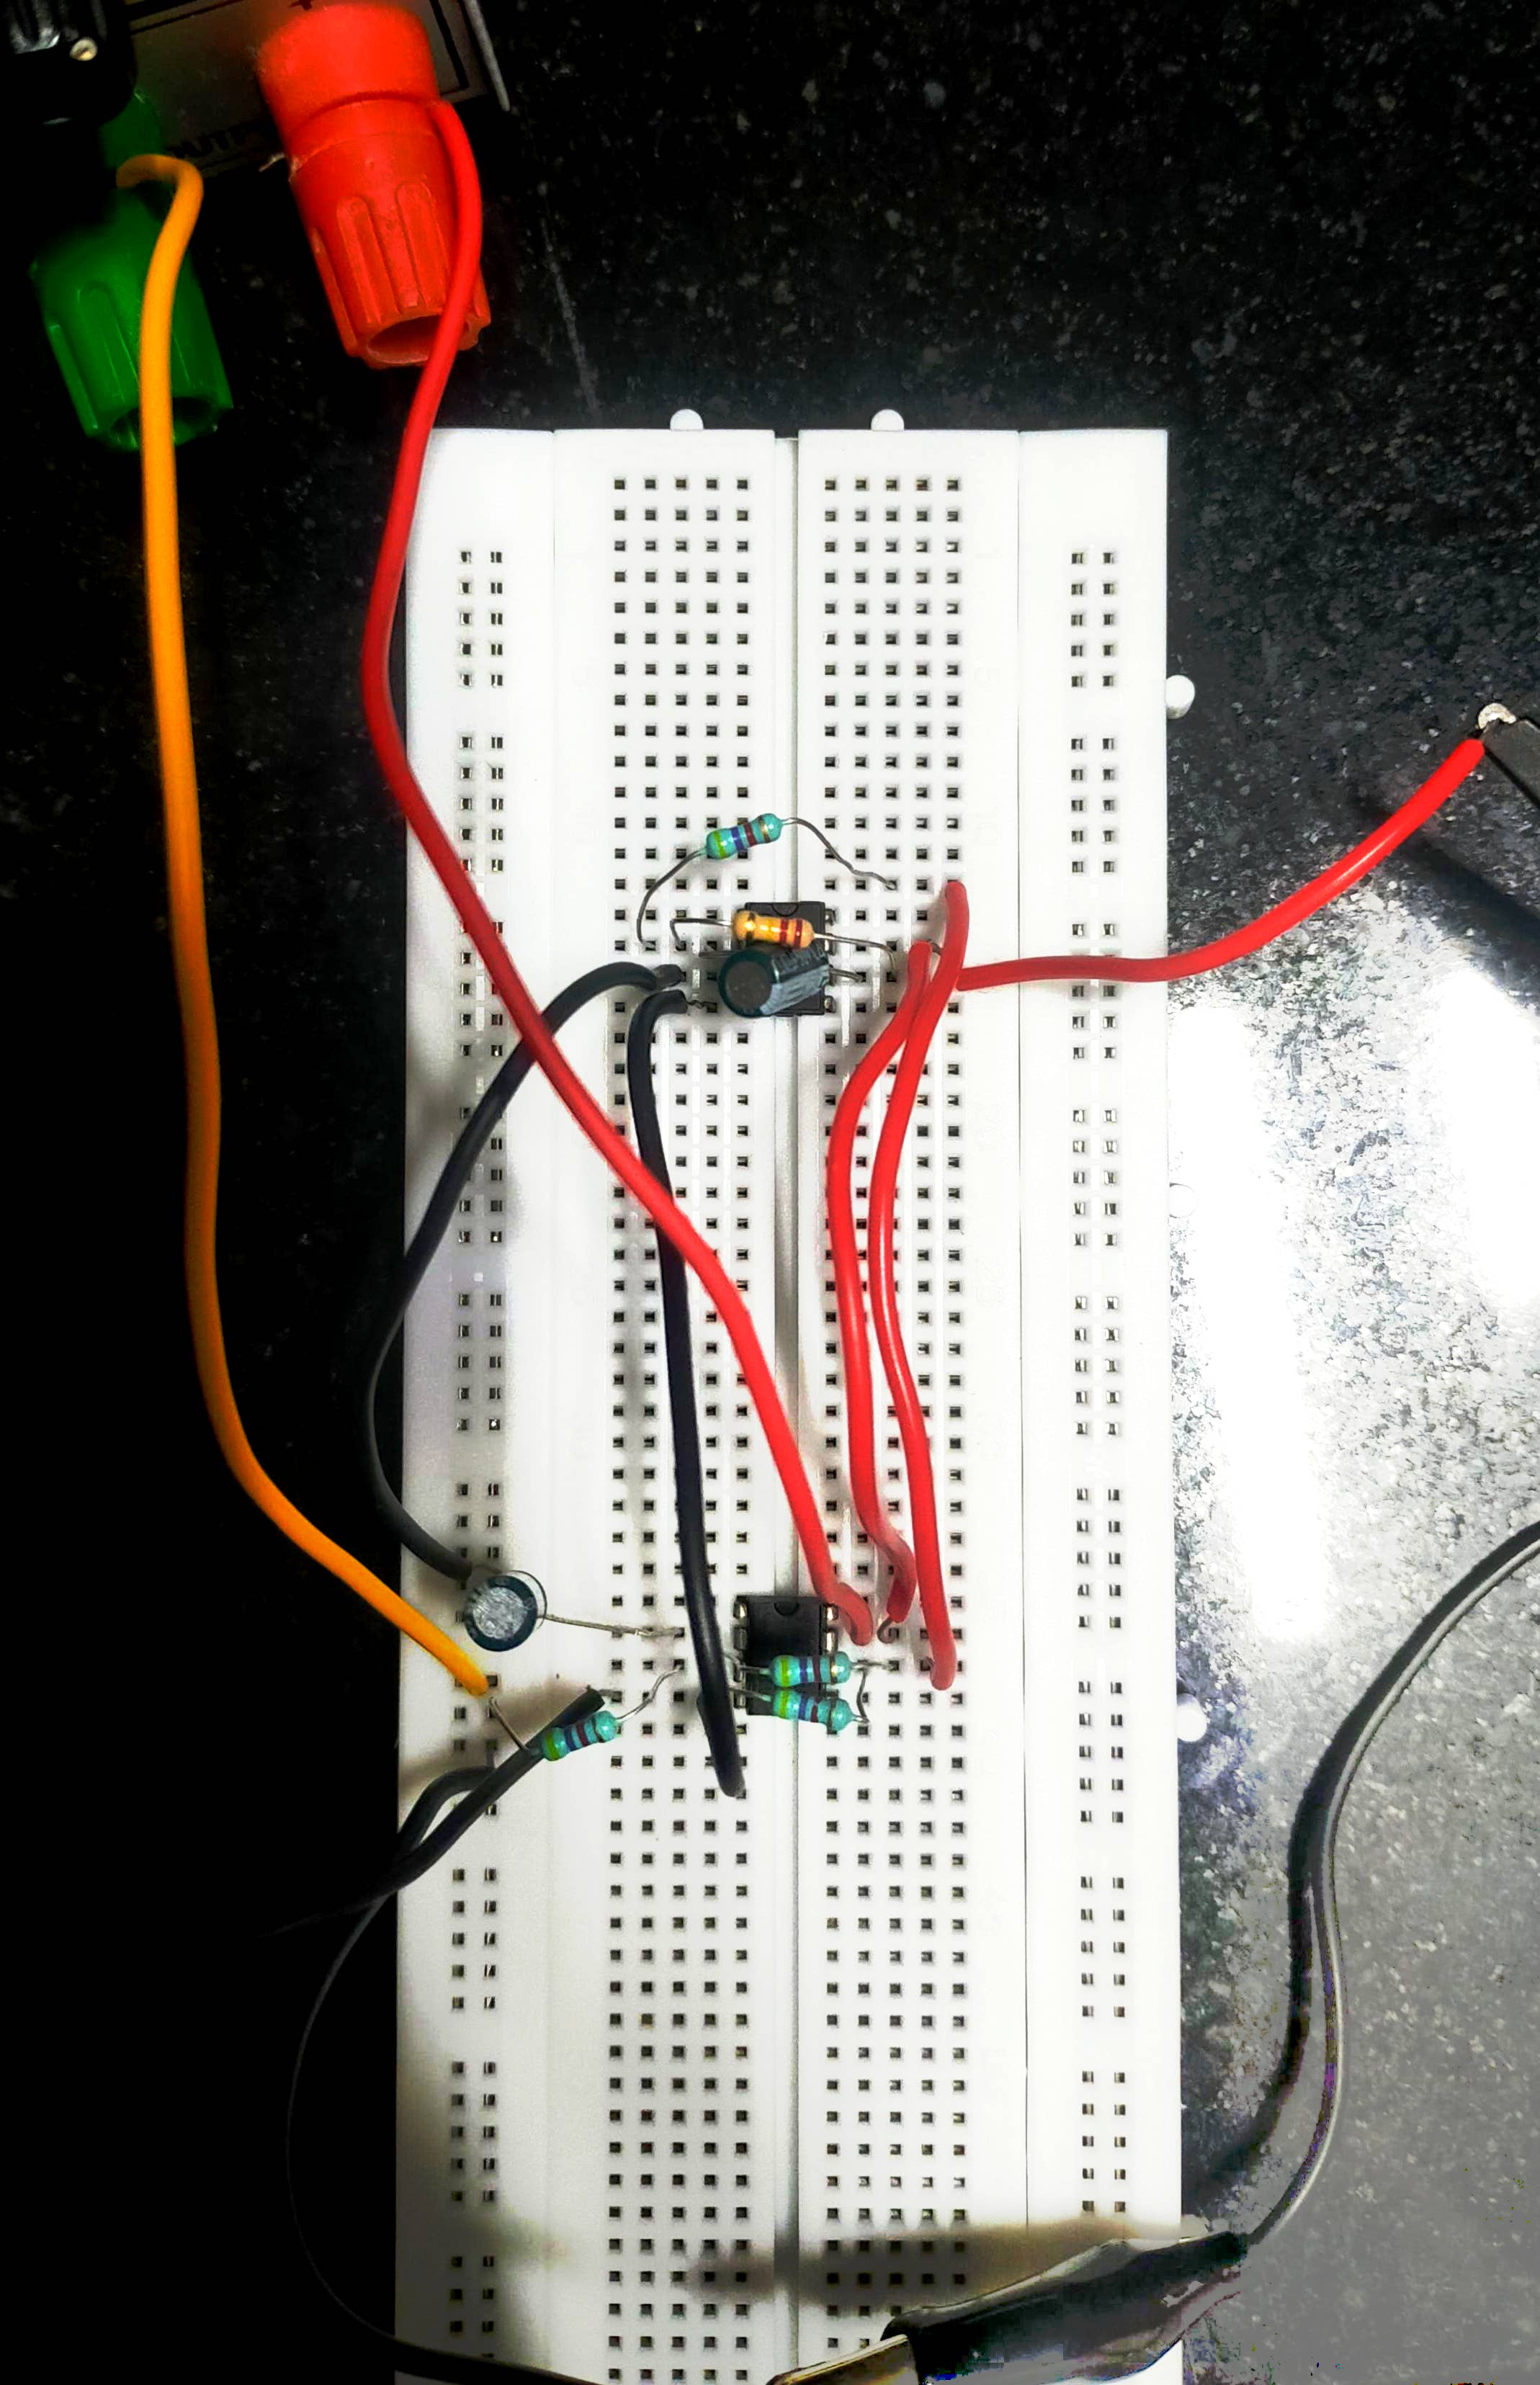
\includegraphics[width=\linewidth]{Images/Triangluar.jpg}
    \caption{Breadboard Circuit Implementation}
    \label{fig:tri_photo}
\end{subfigure}
\hfill
\begin{subfigure}{0.48\textwidth}
    \centering
    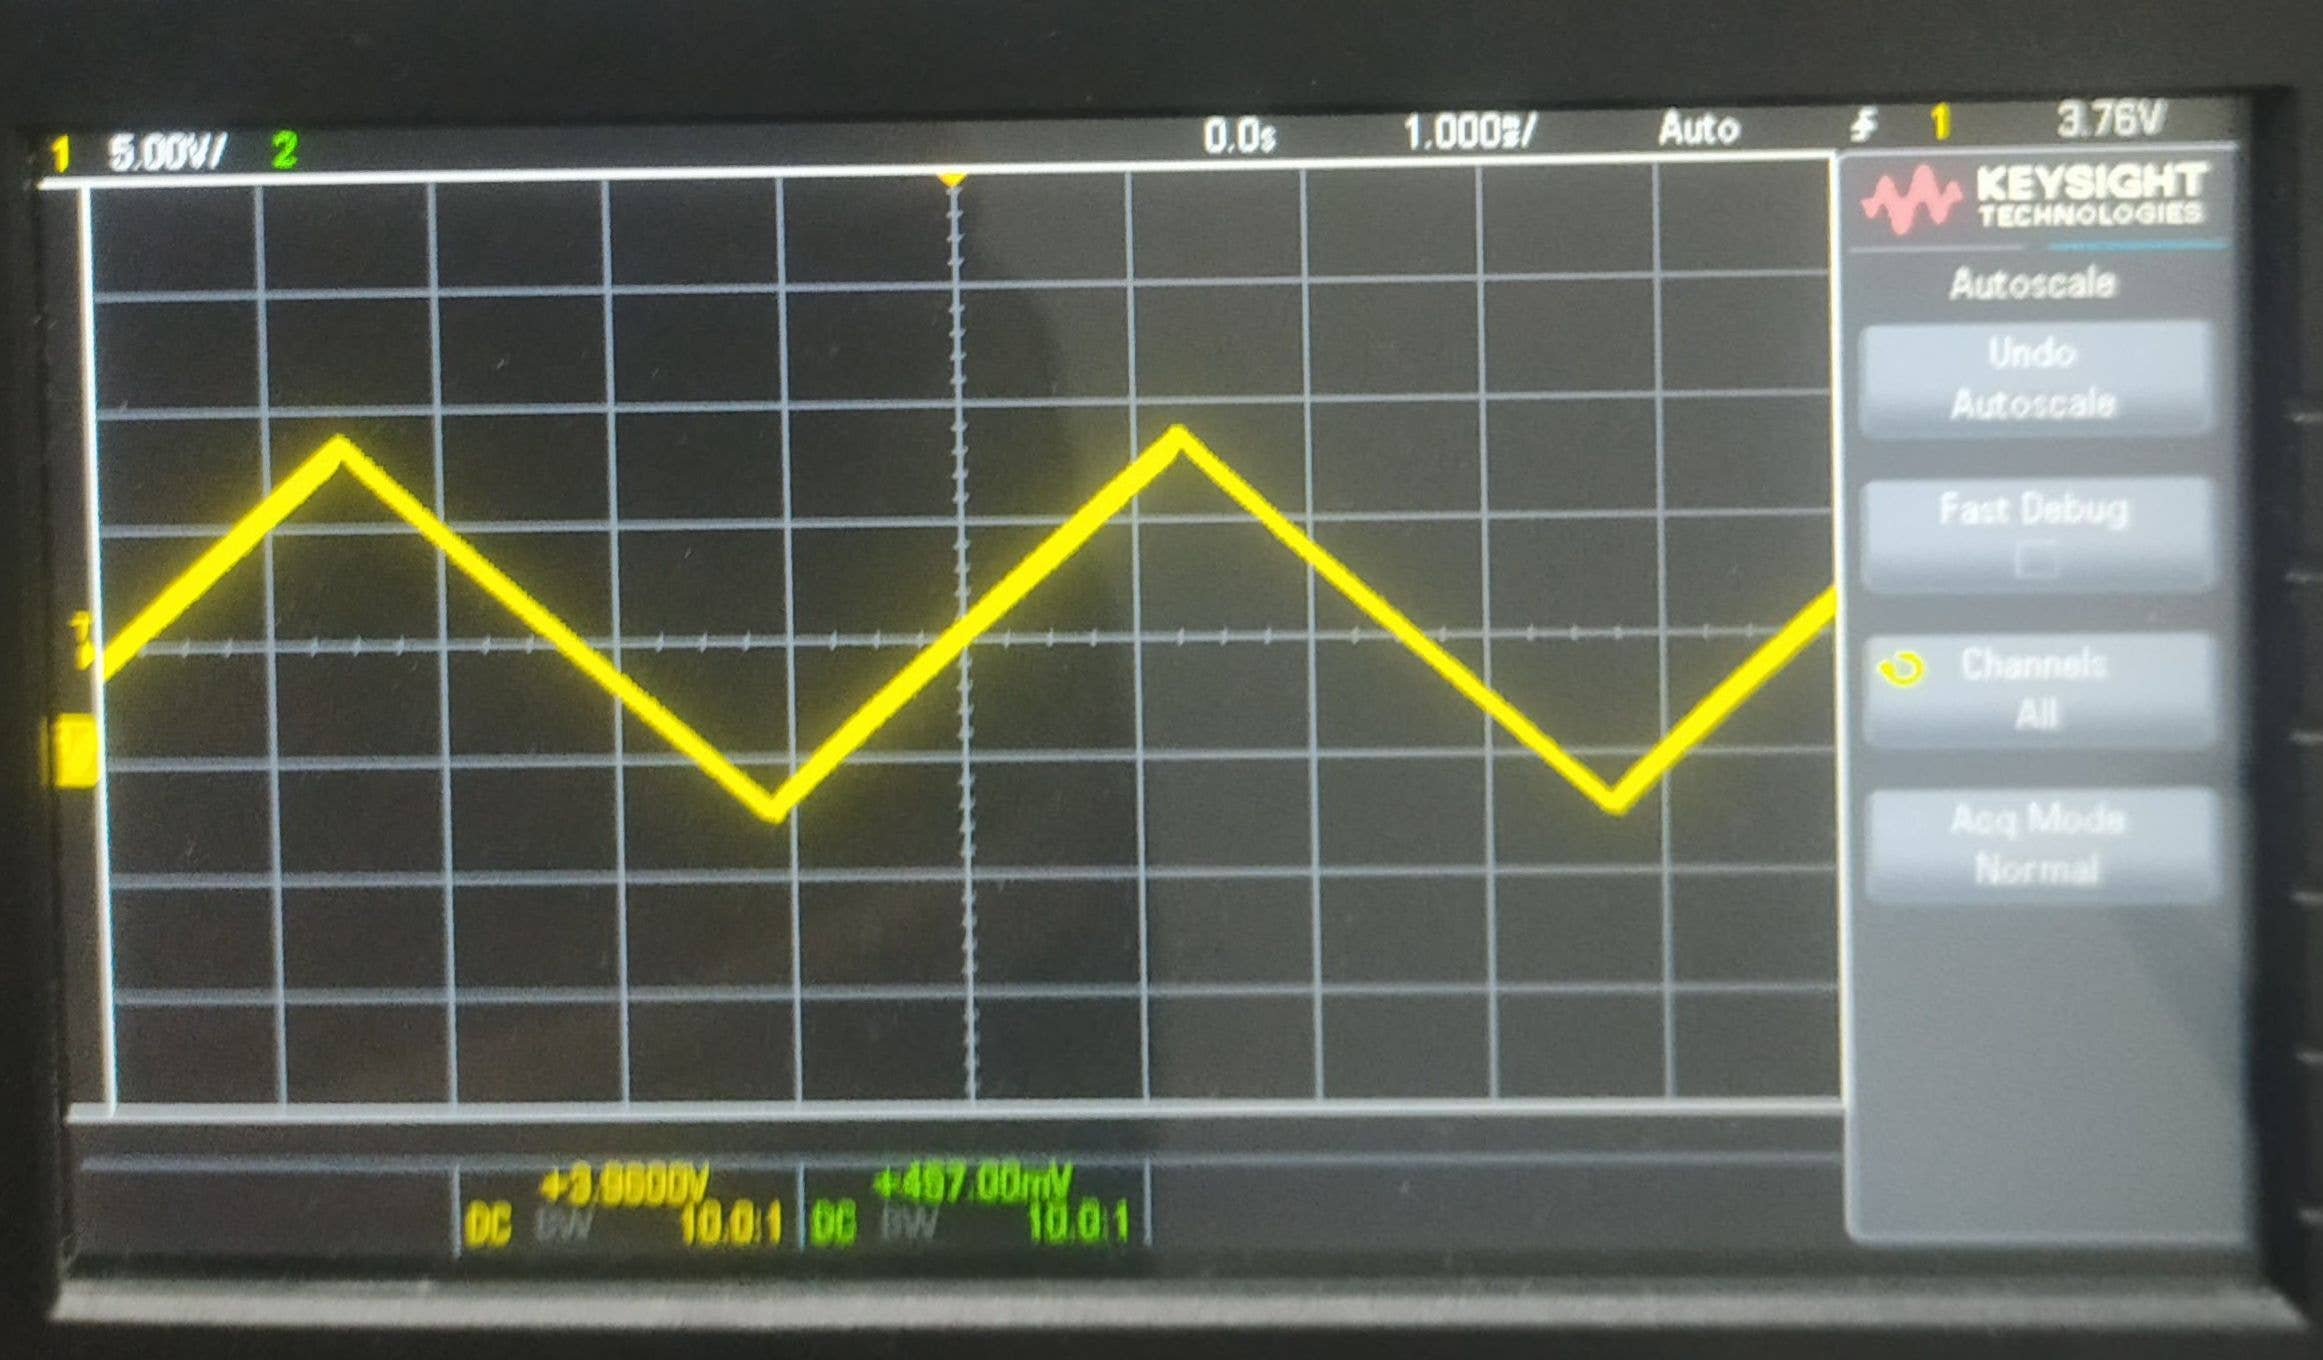
\includegraphics[width=\linewidth]{Images/Graph_Triangular.jpg}
    \caption{Oscilloscope Signal Capture}
    \label{fig:tri_graph}
\end{subfigure}
\caption{Experimental setup and oscilloscope capture of the triangle wave generator output.}
\label{fig:exp_triangle}
\end{figure}

\subsection{Sawtooth Wave Circuit}
By applying an adjustable DC bias voltage at Pin 3 using the potentiometer and changing the input resistor to $33\text{ k}\Omega$, the charging and discharging rates became uneven. As seen in Figure~\ref{fig:exp_sawtooth}, the waveform transformed into a sawtooth wave with a gradual upward slope and a sharp downward drop.

\begin{figure}[H]
\centering
\begin{subfigure}{0.48\textwidth}
    \centering
    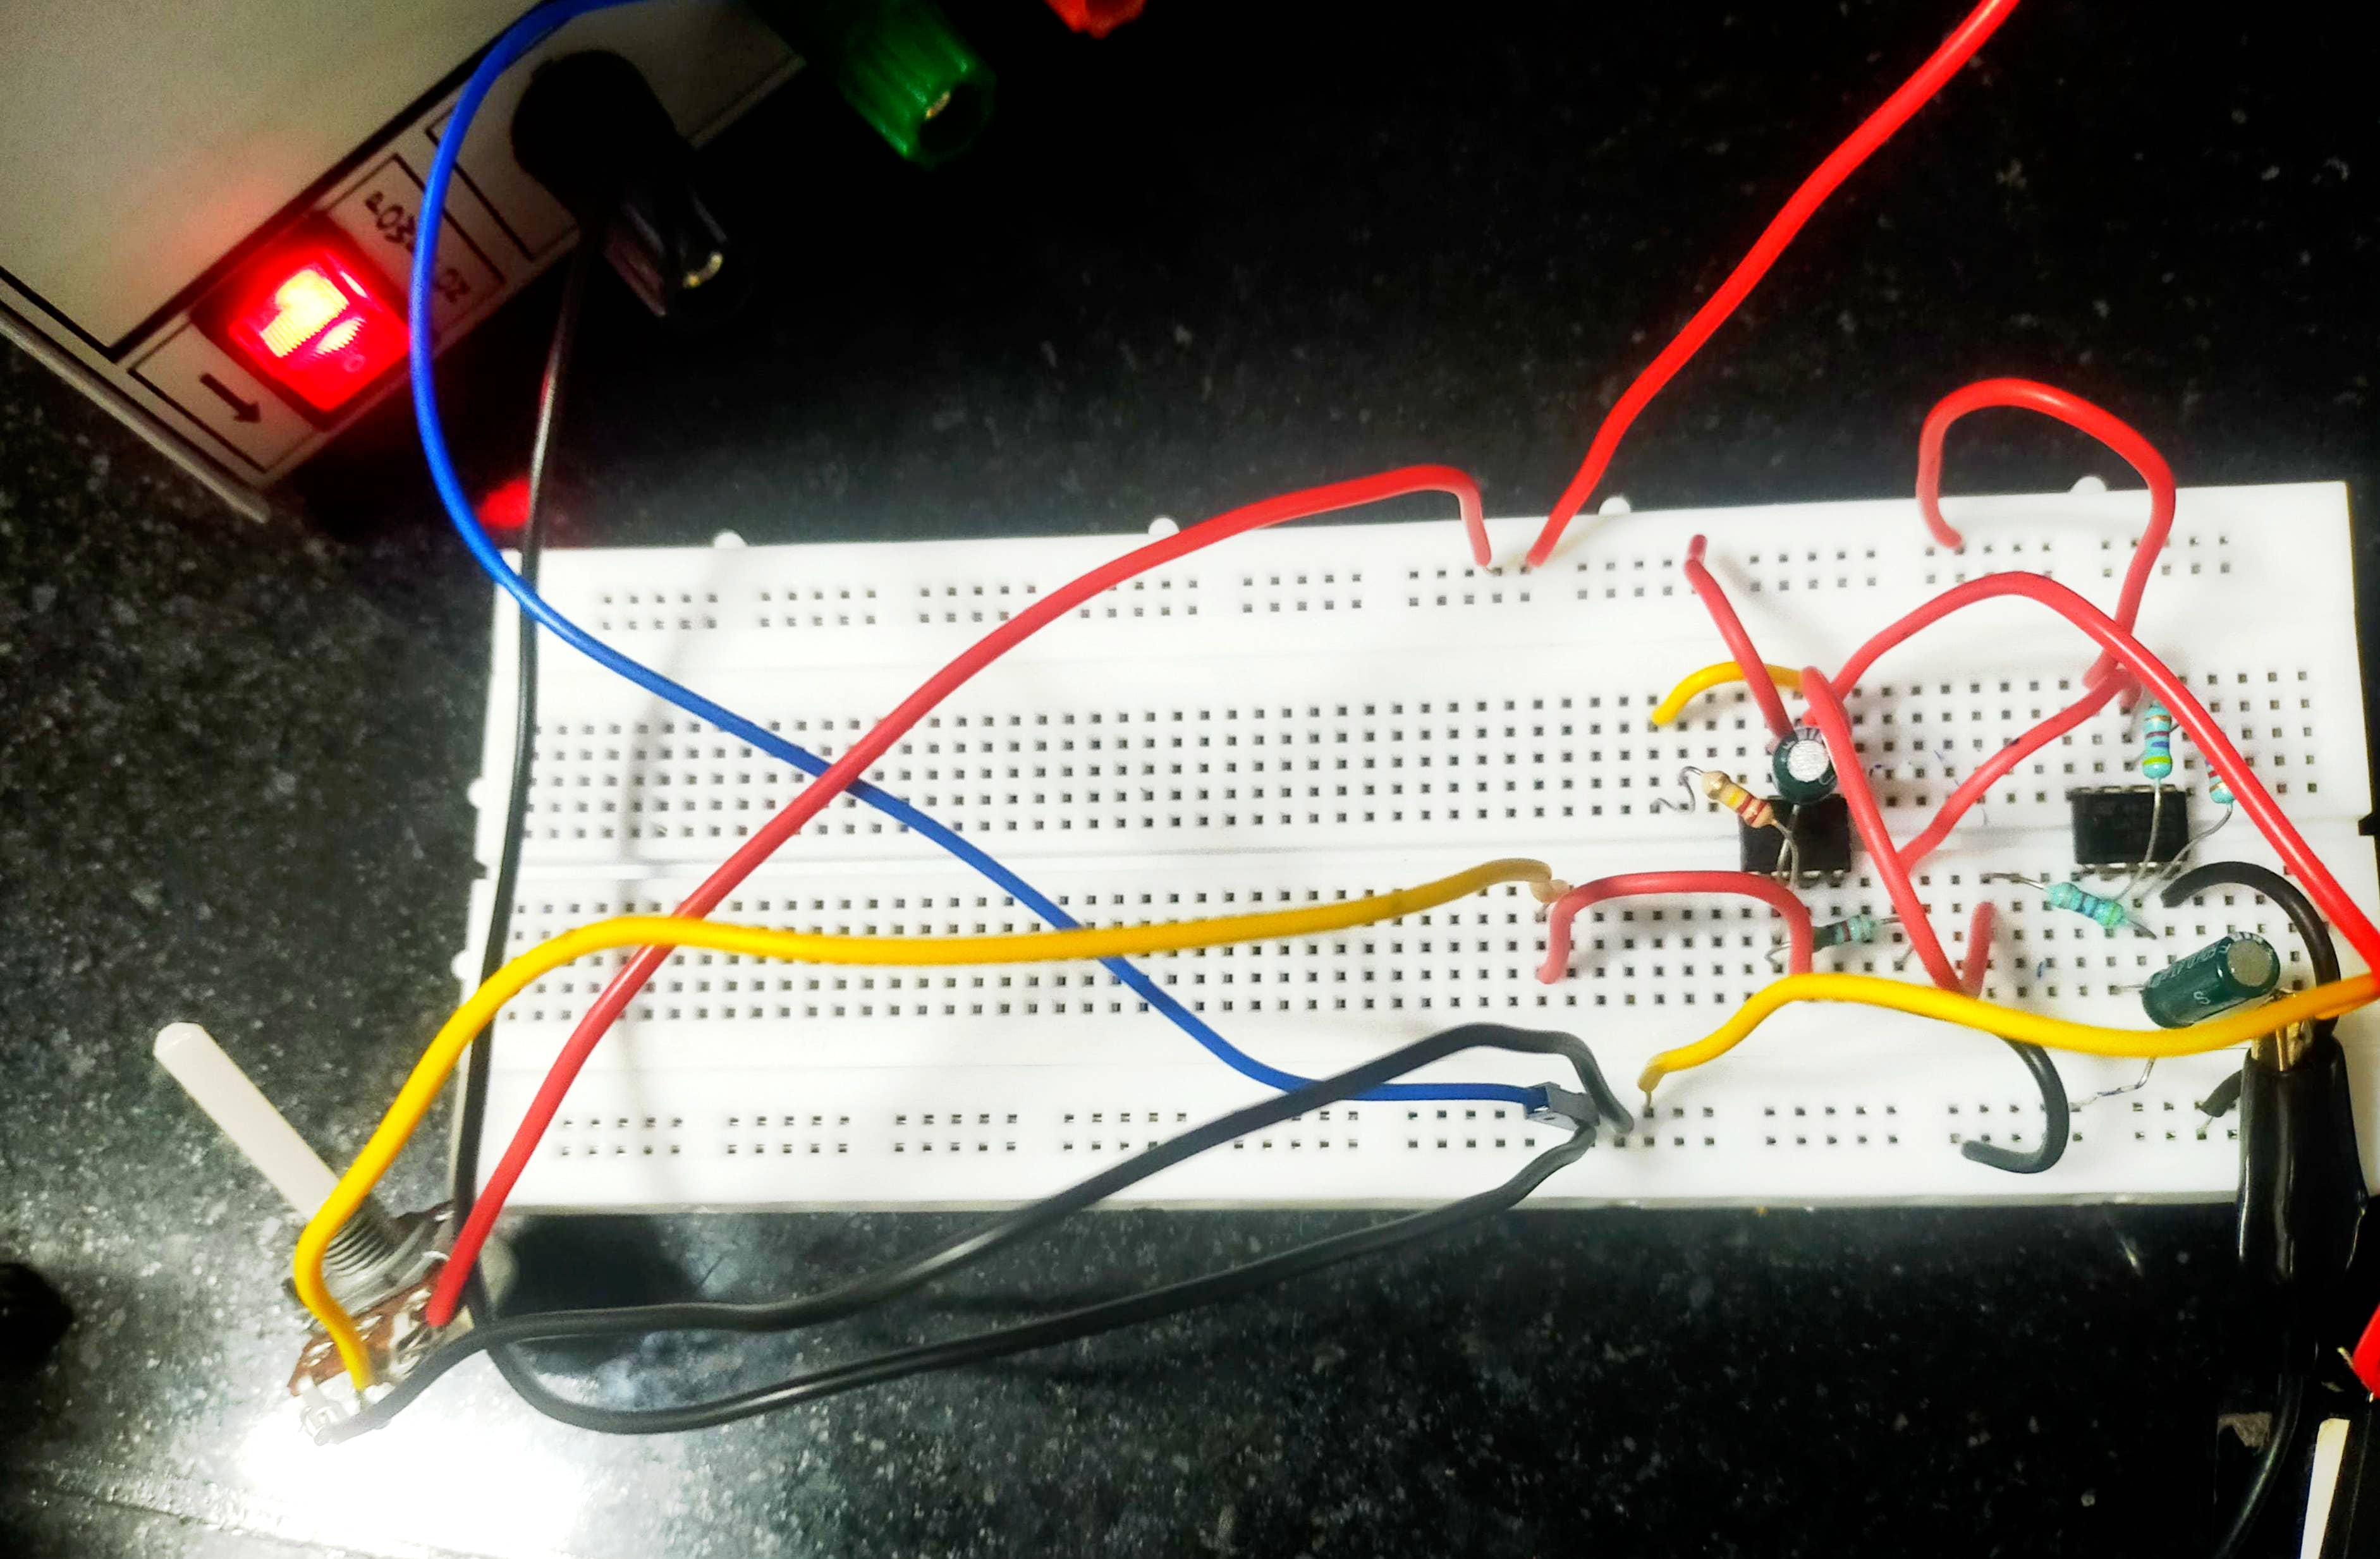
\includegraphics[width=\linewidth]{Images/SawTooth.jpg}
    \caption{Breadboard Circuit Implementation}
    \label{fig:saw_photo}
\end{subfigure}
\hfill
\begin{subfigure}{0.48\textwidth}
    \centering
    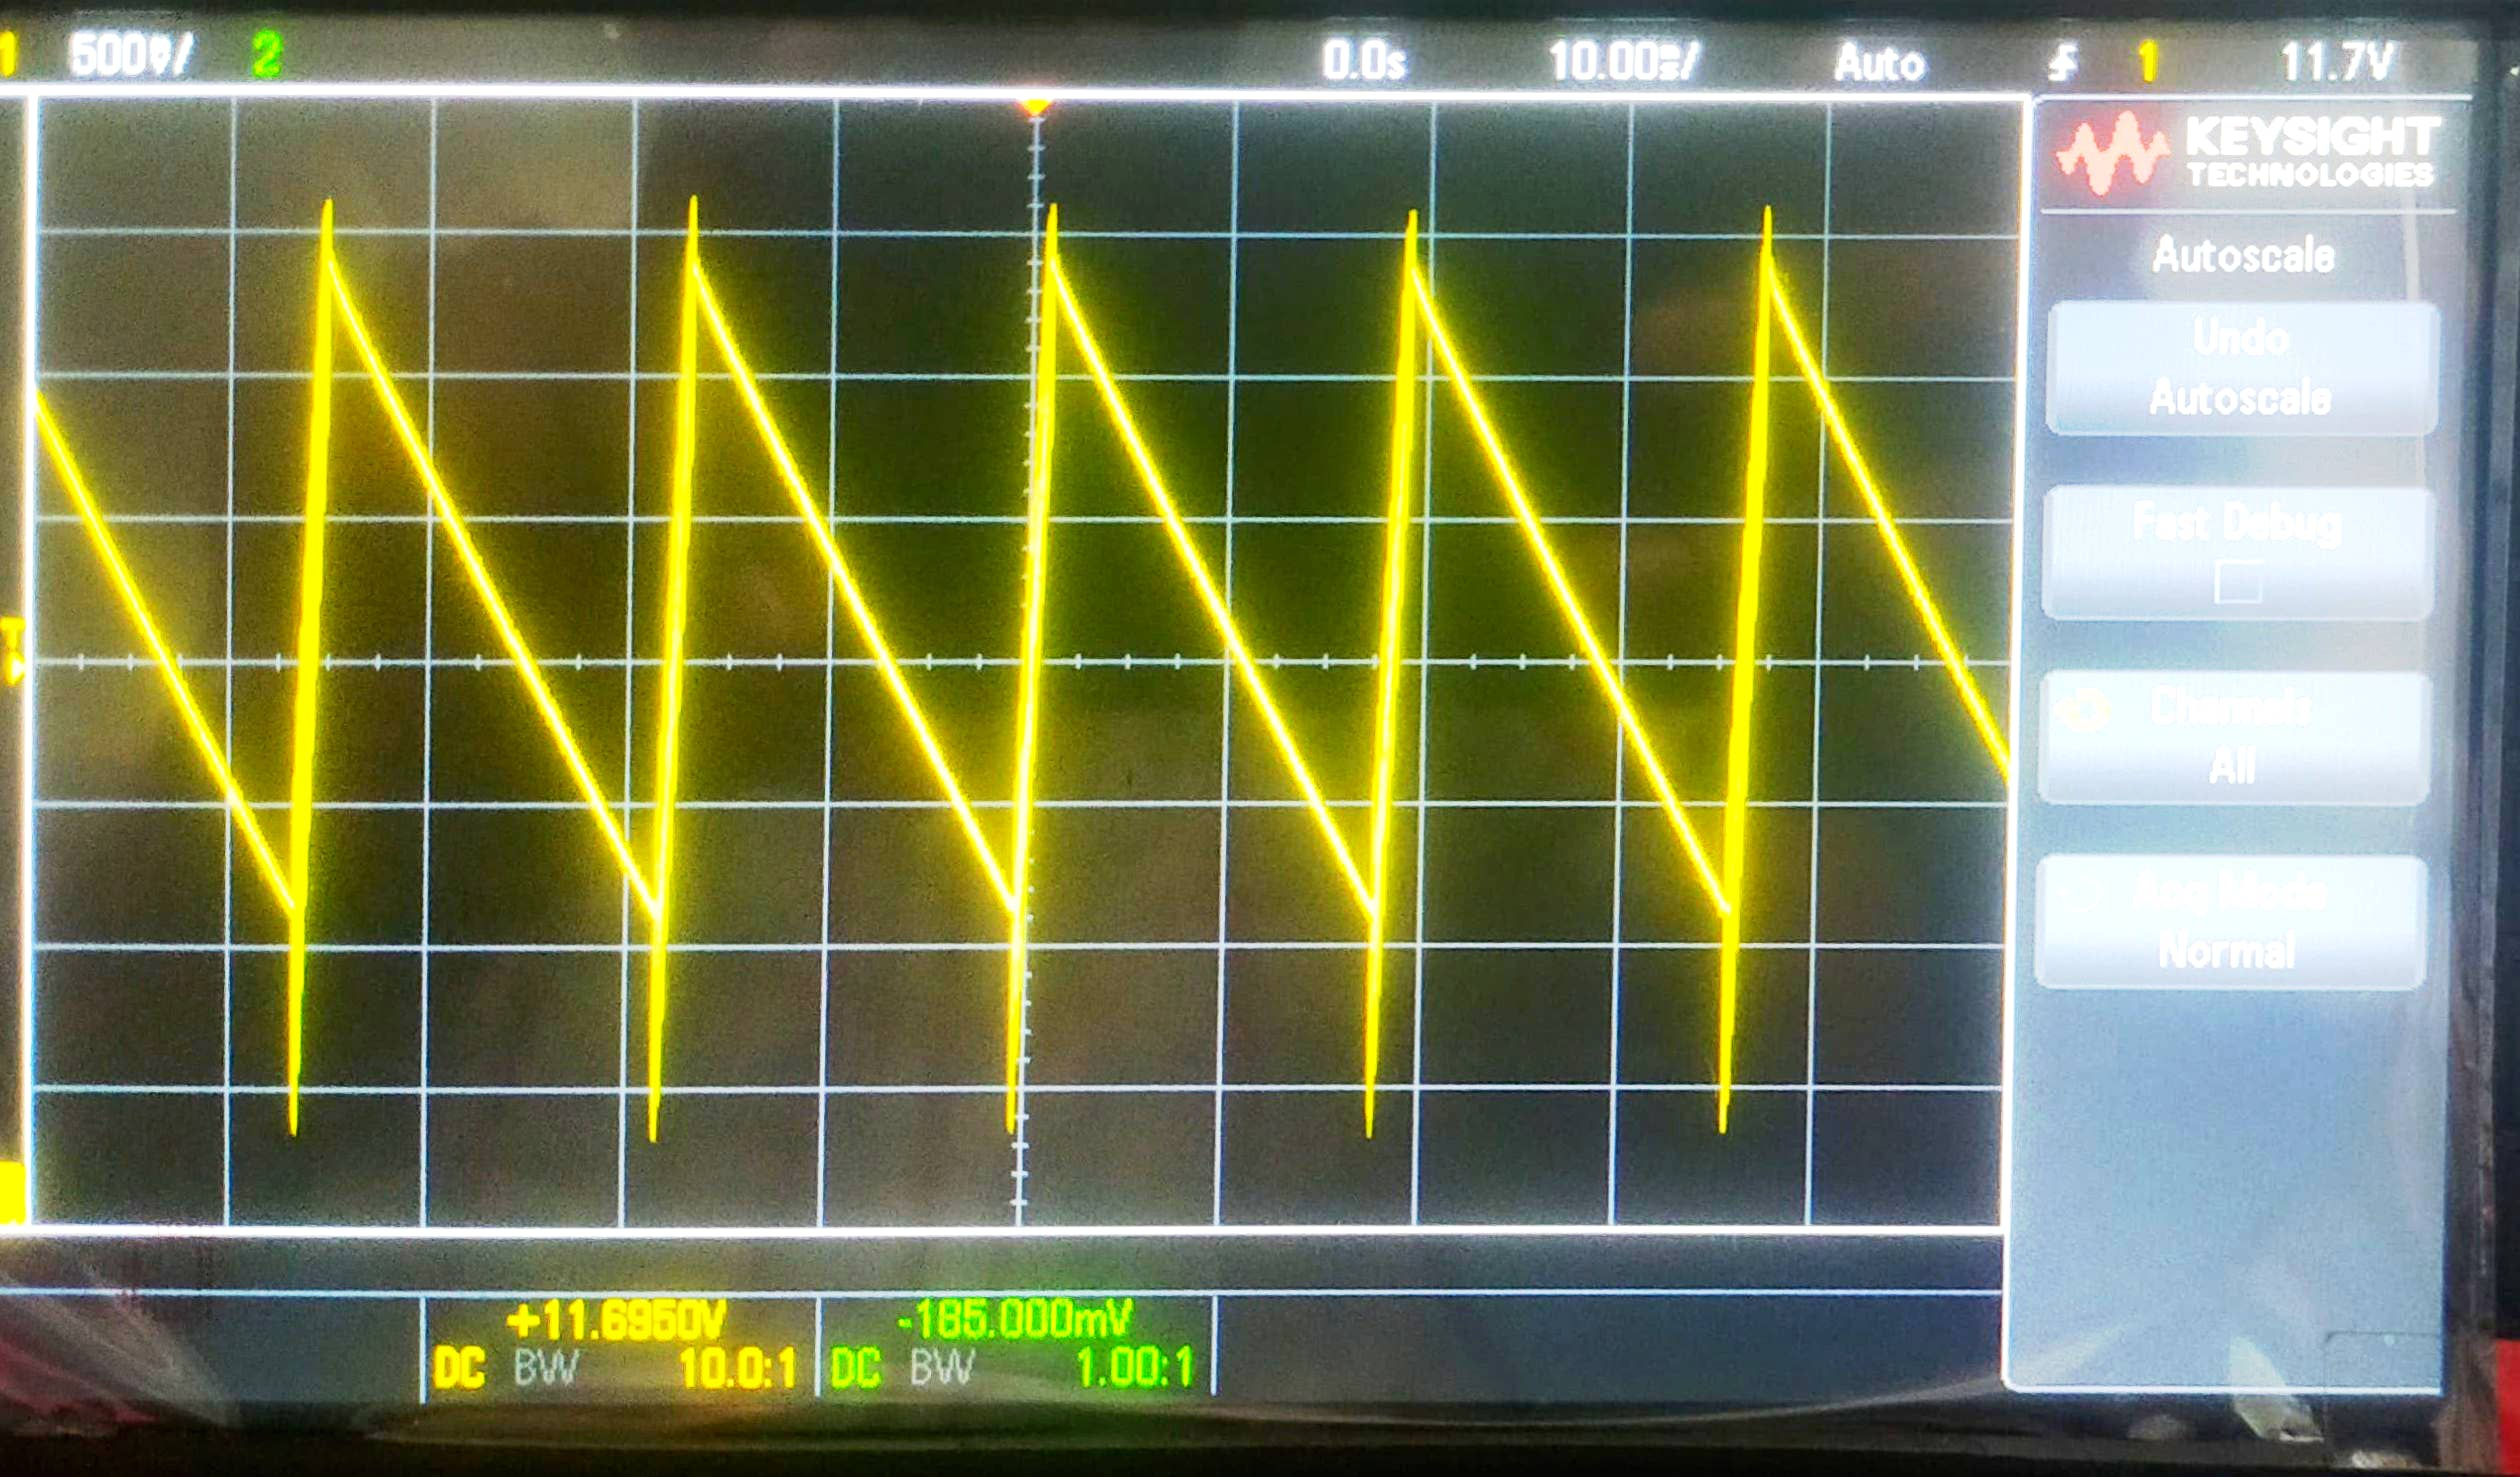
\includegraphics[width=\linewidth]{Images/Graph_Sawtooth.jpg}
    \caption{Oscilloscope Signal Capture}
    \label{fig:saw_graph}
\end{subfigure}
\caption{Experimental setup and oscilloscope capture of the sawtooth wave generator output.}
\label{fig:exp_sawtooth}
\end{figure}

% ==========================================
% 6. OBSERVATIONS & TROUBLESHOOTING
% ==========================================
\section{Observations and Troubleshooting}

\subsection{Observed and Theoretical Time Periods}
Table~\ref{tab:time_periods} compares the theoretical time periods calculated from component values ($T_{\text{theo}} \approx 2.2RC$) against the actual time periods ($T_{\text{obs}}$) and frequencies measured on the oscilloscope.

\begin{table}[H]
\centering
\caption{Comparison of Theoretical vs. Observed Time Periods and Frequencies}
\label{tab:time_periods}
\renewcommand{\arraystretch}{1.4}
\begin{tabular}{lcccc}
\toprule
\textbf{Waveform} & \textbf{$T_{\text{theoretical}}$} & \textbf{$T_{\text{observed}}$} & \textbf{$f_{\text{observed}}$} & \textbf{Error (\%)} \\
\midrule
Square Wave (Astable) & $4.86\text{ ms}$ & $4.90\text{ ms}$ & $204.1\text{ Hz}$ & $0.82\%$ \\[2mm]
Triangle Wave (Integrator) & $4.86\text{ ms}$ & $4.90\text{ ms}$ & $204.1\text{ Hz}$ & $0.82\%$ \\[2mm]
Sawtooth Wave (Biased Int.) & $4.86\text{ ms}$ & $4.375\text{ ms}$ & $228.6\text{ Hz}$ & $9.98\%$ \\
\bottomrule
\end{tabular}
\end{table}


\subsection{Circuit Behavior and Troubleshooting}
During the setup and testing of the circuits, a few practical behaviors and common measurement issues were observed and resolved:

\begin{itemize}
    \item \textbf{Probing the Input vs. Output:} Connecting the probe to Pin 2 (the inverting input) of the square wave generator instead of Pin 6 shows an exponential charging and discharging voltage instead of a square wave. This occurs because Pin 2 monitors the voltage across the timing capacitor $C$. To view the true square wave signal, the probe must be connected to the op-amp output on Pin 6.
    
    \item \textbf{Oscilloscope Coupling Mode:} If the oscilloscope channel is set to AC coupling instead of DC coupling, an internal capacitor is placed in series with the input signal. At around $200\text{ Hz}$, this acts like a high-pass filter and turns the flat square wave into sharp voltage spikes (differentiation). The oscilloscope must be set to \textbf{DC coupling} to view the correct waveform shape.
    
    \item \textbf{Incorrect Timebase Setting:} If the oscilloscope timebase is set too slow (such as $2.0\text{ s/div}$) while viewing a $200\text{ Hz}$ signal, the screen samples too slowly and displays a distorted, stepped ``staircase'' wave. Adjusting the horizontal timebase to $1\text{--}2\text{ ms/div}$ cleanly solves this issue and correctly displays the true wave shape.
    
    \item \textbf{Op-Amp Saturation (Clipping):} When initially testing the sawtooth circuit using a smaller input resistor ($R_{in} = 4.7\text{ k}\Omega$), too much current entered the integrator. This caused the voltage to rise too fast and hit the $\pm 15\text{V}$ power supply limits, flattening the tops and bottoms of the waveform (clipping). Increasing the input resistor to $33\text{ k}\Omega$ slowed down the charging current, keeping the voltage within operational limits and restoring clean sawtooth peaks.
\end{itemize}

% ==========================================
% 7. RESULTS & CONCLUSION
% ==========================================
\section{Results and Conclusion}
In this experiment, three operational amplifier waveform generator circuits were successfully assembled and tested using the IC 741:
\begin{enumerate}
    \item A stable \textbf{square wave} was generated using an op-amp configured as an astable multivibrator, with an observed time period ($4.90\text{ ms}$) closely matching the theoretical calculation ($4.86\text{ ms}$).
    \item A clean \textbf{triangle wave} was produced by passing the square wave through an integrator circuit. A $220\text{ k}\Omega$ feedback resistor proved necessary to prevent offset voltage drift and keep the signal centered about zero volts.
    \item An adjustable \textbf{sawtooth wave} was created by applying a variable DC bias voltage to Pin 3 of the integrator using a potentiometer and increasing the input resistor to $33\text{ k}\Omega$, demonstrating how voltage biasing effectively controls wave asymmetry.
\end{enumerate}

\end{document}
